\begin{ledgroupsized}[r]{120mm}
\footnotesize 
\pstart 
\noindent\textbf{\"{U}berlieferung:}
\pend
\end{ledgroupsized}
\begin{ledgroupsized}[r]{114mm}
\footnotesize 
\pstart \parindent -6mm
\makebox[6mm][l] {\textit{L}} Konzept: LH XXXV 13, 3 Bl. 35. 1 Bl. 26 x 24 cm. 1 S. Text auf Bl. 35 v\textsuperscript{o}; r\textsuperscript{o}-Seite leer. Linker und unterer Rand beschnitten. Der untere Rand folgt dem Schriftbefund und uml\"{a}uft [\textit{Fig. 5}] links unten in einer S-f\"{o}rmigen Kurve. S\"{a}mtliche Zeichnungen am linken Rand. Die Marginalie bezieht sich auf [\textit{Fig. 3}], wobei der Schriftverlauf die Grafik vollst\"{a}ndig umschlie{\ss}t. In der dritten Zeile von unten befinden sich Wortfragmente, die aufgrund fehlenden Bezuges zum Text unber\"{u}cksichtigt bleiben. In derselben Zeile eine nicht zum Text geh\"{o}rende und getilgte Passage. Wasserzeichen nahe des unteren Randes. \\Cc 2 Nr. 974 \pend
\end{ledgroupsized}
 
\vspace*{5mm}
\begin{ledgroup}
\footnotesize 
\pstart
\noindent\footnotesize{\textbf{Datierungsgr\"{u}nde}: Ein Hinweis \"{u}ber die Entstehungszeit dieses St\"{u}ckes ergibt sich aus der Zeichnung [\textit{Fig. 4}], welche auch andernorts in Leibniz' Schriftcorpus vorkommt, n\"{a}mlich: 1) in einem Auszug aus Wallis' \textit{De Motu} (N. ??), der sich auf die zweite H\"{a}lfte des Jahres 1674 datieren l\"{a}sst (dort wird das Bild ebenfalls beim Nachweis der Unm\"{o}glichkeit eines perpetuum mobile angef\"{u}hrt); 2) auf LH XXXV 2, 1 Bl. 273~v\textsuperscript{o}, in einem St\"{u}ck \"{u}ber die geometrische Beschreibung transzendenter Quadratrices (Cc 2 Nr. 897), das aufgrund des inhaltlichen Zusammenhangs mit dem vom Leibniz eigenh\"{a}ndig datierten St\"{u}ck Cc 2 Nr. 895 sp\"{a}testens im Januar 1675 verfasst worden sein muss; 3) im St\"{u}ck \textit{De detrimento motus. Pars prima} (N. ??R/a\textsubscript{1}), das auf sp\"{a}testens April 1675 datiert werden kann (an beiden letzteren Stellen weist die Zeichnung allerdings keinen unmittelbar erkennbaren Zusammenhang mit dem jeweiligen Text auf). Ferner ist das auf Bl. 35~v\textsuperscript{o} anzutreffende Wasserzeichen f\"{u}r April 1675 belegt. Demgem\"{a}{\ss} l\"{a}sst sich f\"{u}r das vorliegende St\"{u}ck ein Entstehungszeitraum zwischen Sommer 1674 und April 1675 als plausibel annehmen. Diese Datierung wird durch das WZ gut best\"{a}tigt, das ausf\"{u}hrlich und pr\"{u}zise auf April bis Juni 1675 datiert ist.}
\pend
\end{ledgroup}

\vspace*{8mm}
\pstart 
\normalsize
[35 v\textsuperscript{o}] \pend \pstart
\begin{wrapfigure}{l}{0.6\textwidth}  
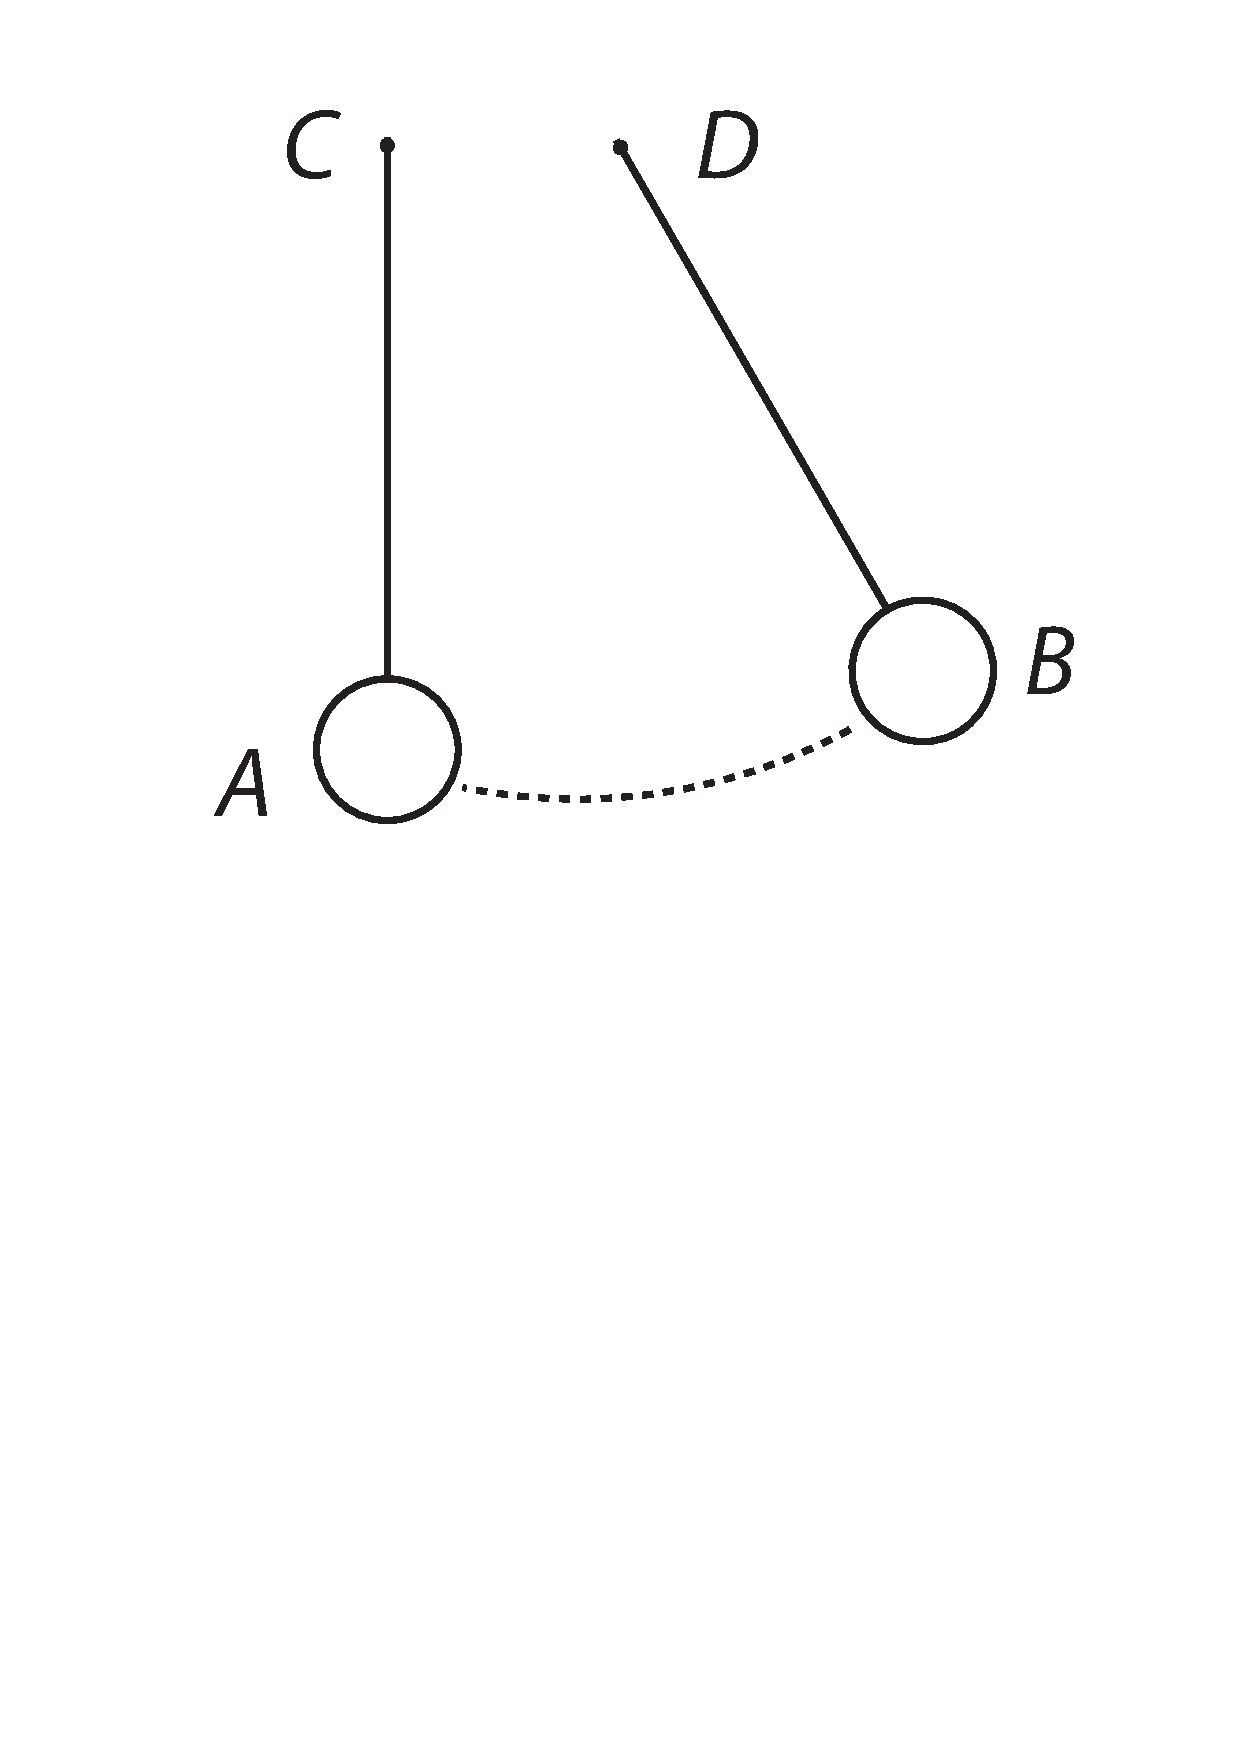
\includegraphics[width=0.23\textwidth] {images/lh0351303_035r-d1.pdf}\rule[0cm]{13mm}{0cm}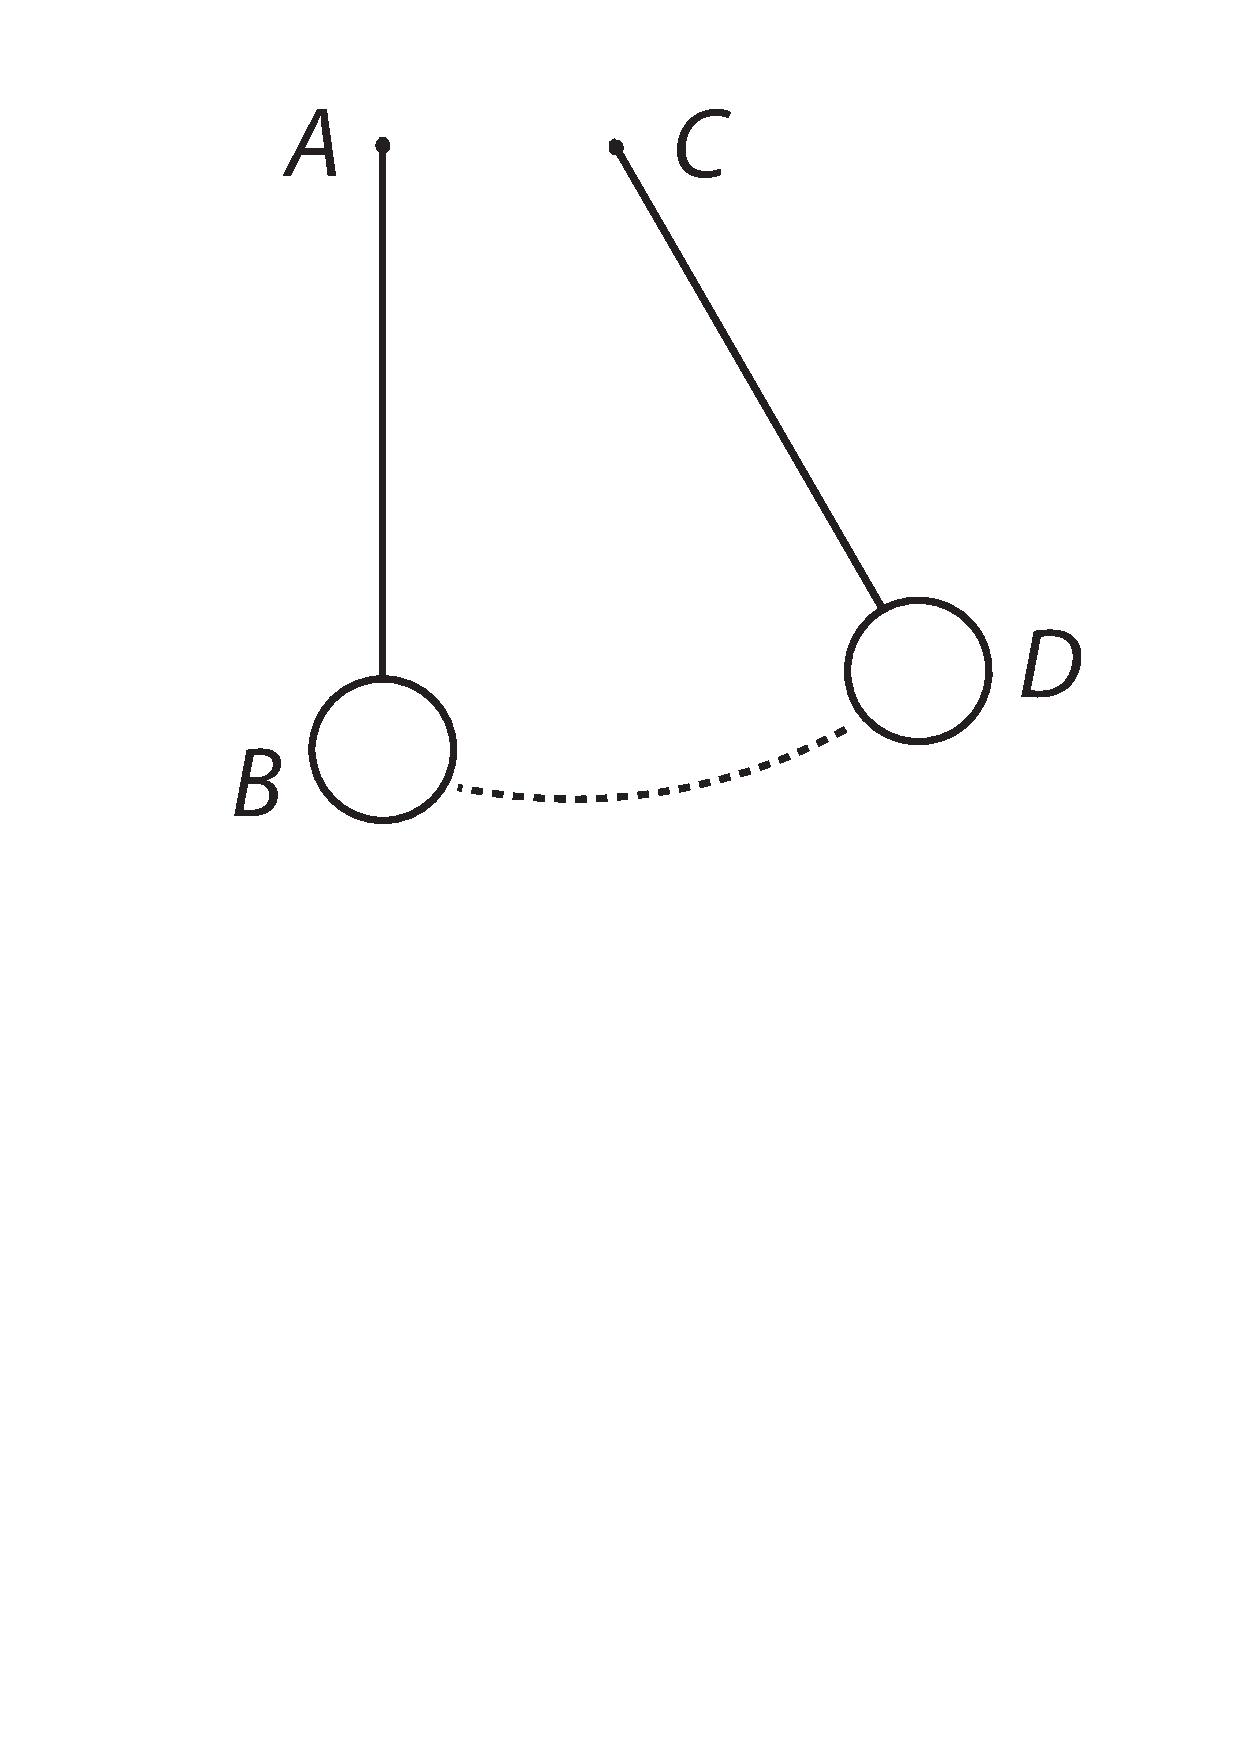
\includegraphics[width=0.23\textwidth] {images/lh0351303_035r-d2.pdf}\\
\rule[0cm]{1mm}{0cm}\textit{[Fig. 1, gestrichen]} \rule[0cm]{20mm}{0cm}\textit{[Fig. 2]}
\end{wrapfigure} Si Motus non nisi situs mutatio esset, (: quod non Cartesium\protect\index{Namensregister}{\textso  {Descartes}, Ren\´{e} (1596-1650)} tantum sed et Hugenium\protect\index{Namensregister}{\textso  {Huygens}, Christiaan (1629-1695)} sentire video :) duobus corporibus sibi appropinquantibus nihil referret, alterum an utrumque, \edtext{ac si alterutrum, quodnam ex ipsis, mover}{\lemma{utrumque} \Bfootnote{ \textit{ (1) }\ moveretur a \textit{ (2) }\ ac si alterutrum, quodnam ex ipsis, moveri \textit{ L}\ }} dicatur. Unde pendulum \textit{CD} impingat in pendulum \textit{AB} perinde erit ac si alterum alteri occurreret, \edtext{aequali celeritate unde}{\lemma{occurreret} \Bfootnote{ \textit{ (1) }\ unde aliamque \textit{ (2) }\ aequali celeritate unde \textit{ L}\ }} quiesceret utrumque, quod est experientiae adversum. Nam (si nullum adsit Elaterium) pendulum \textit{AB} a pendulo \textit{CD} nulla motus sui diminutione aufertur. \edtext{Responderi potest huic objectioni pro definitione motus}{\lemma{aufertur.} \Bfootnote{ \textit{ (1) }\ Sed his responderi potest, etsi motus h \textit{ (2) }\ Responderi potest  \textbar , \textit{streicht Hrsg.} \textbar  huic objectioni pro definitione motus \textit{ L }\ }} a qua nec ego abhorreo, non de motu hic sed de effectu esse quaestionem, et cum quidlibet fingi possit pro arbitrio, motum generalem exitum quem potest reperire. \\
Pone \( \displaystyle AB \, \sqcap \, x \, \sqcap \, GW \, \sqcap \, z \). \edtext{ \( \displaystyle WL \, \sqcap \, \dfrac{ a \beta }{ x } \) }{ \lemma{ z.} \Bfootnote{ \textit{ (1) } $  \displaystyle WL \, \sqcap \, \dfrac{ a z }{ x } $ \textit{ (2) } $ \displaystyle WL \, \sqcap \, \dfrac{ z } { x } $ \textit{ (3) } $ \displaystyle WL \, \sqcap \, \dfrac{ a \beta }{ x } $ \textit{ L}}}. Sed si pro \edtext{\textit{z}}{\lemma{si pro} \Bfootnote{ \textit{ (1) }\ $\beta$ \textit{ (2) }\ \textit{z} \textit{ L}\ }}, ponamus \( \displaystyle \dfrac{y}{a} \, \beta \), erit \( \displaystyle x  \, \sqcap \, \dfrac{y^{2}}{2a}\), et \edtext{ \( \displaystyle  WL \, \sqcap \, \dfrac{ \uline{\, a\beta \,}} { \dfrac{y^{2}}{2a} } \, \sqcap \dfrac{2a^{2} \beta}{y^{2}} \) }{\lemma{et} \Bfootnote{ \textit{ (1) } $  \displaystyle WL \, \sqcap \, \dfrac{ \dfrac{a\beta}{a}} { \dfrac{y^{2}}{2a}} $ \textit{ (2) } $ \displaystyle WL \, \sqcap \, {\dfrac{ 2a\beta } { }} $  \textit{ (3) }  $ \displaystyle WL \, \sqcap \, \dfrac{ \uline{\, a\beta \,}} { \dfrac{y^{2}}{2a} } \, \sqcap \dfrac{2a^{2} \beta}{y^{2}} $ \textit{ L}}}. \pend
 \pstart
Ergo curva \textit{AGL} quadratrix Hyperbolae \edtext{intelligi potest, descripta duobus motibus compositis, vel ex}{\lemma{quadratrix Hyperbolae}\Bfootnote{ \textit{ (1) }\ composita \textit{ (2) }\ intelligi potest, \textit{ (a) } ex \textit{ (b) } descripta duobus motibus compositis, vel ex\textit{ L }\ }} uniformi, et uniformiter crescentium reciproco, vel uniformiter crescente, et uniformiter crescentium quadratis reciproco.
\begin{wrapfigure}{l}{0,3\textwidth}
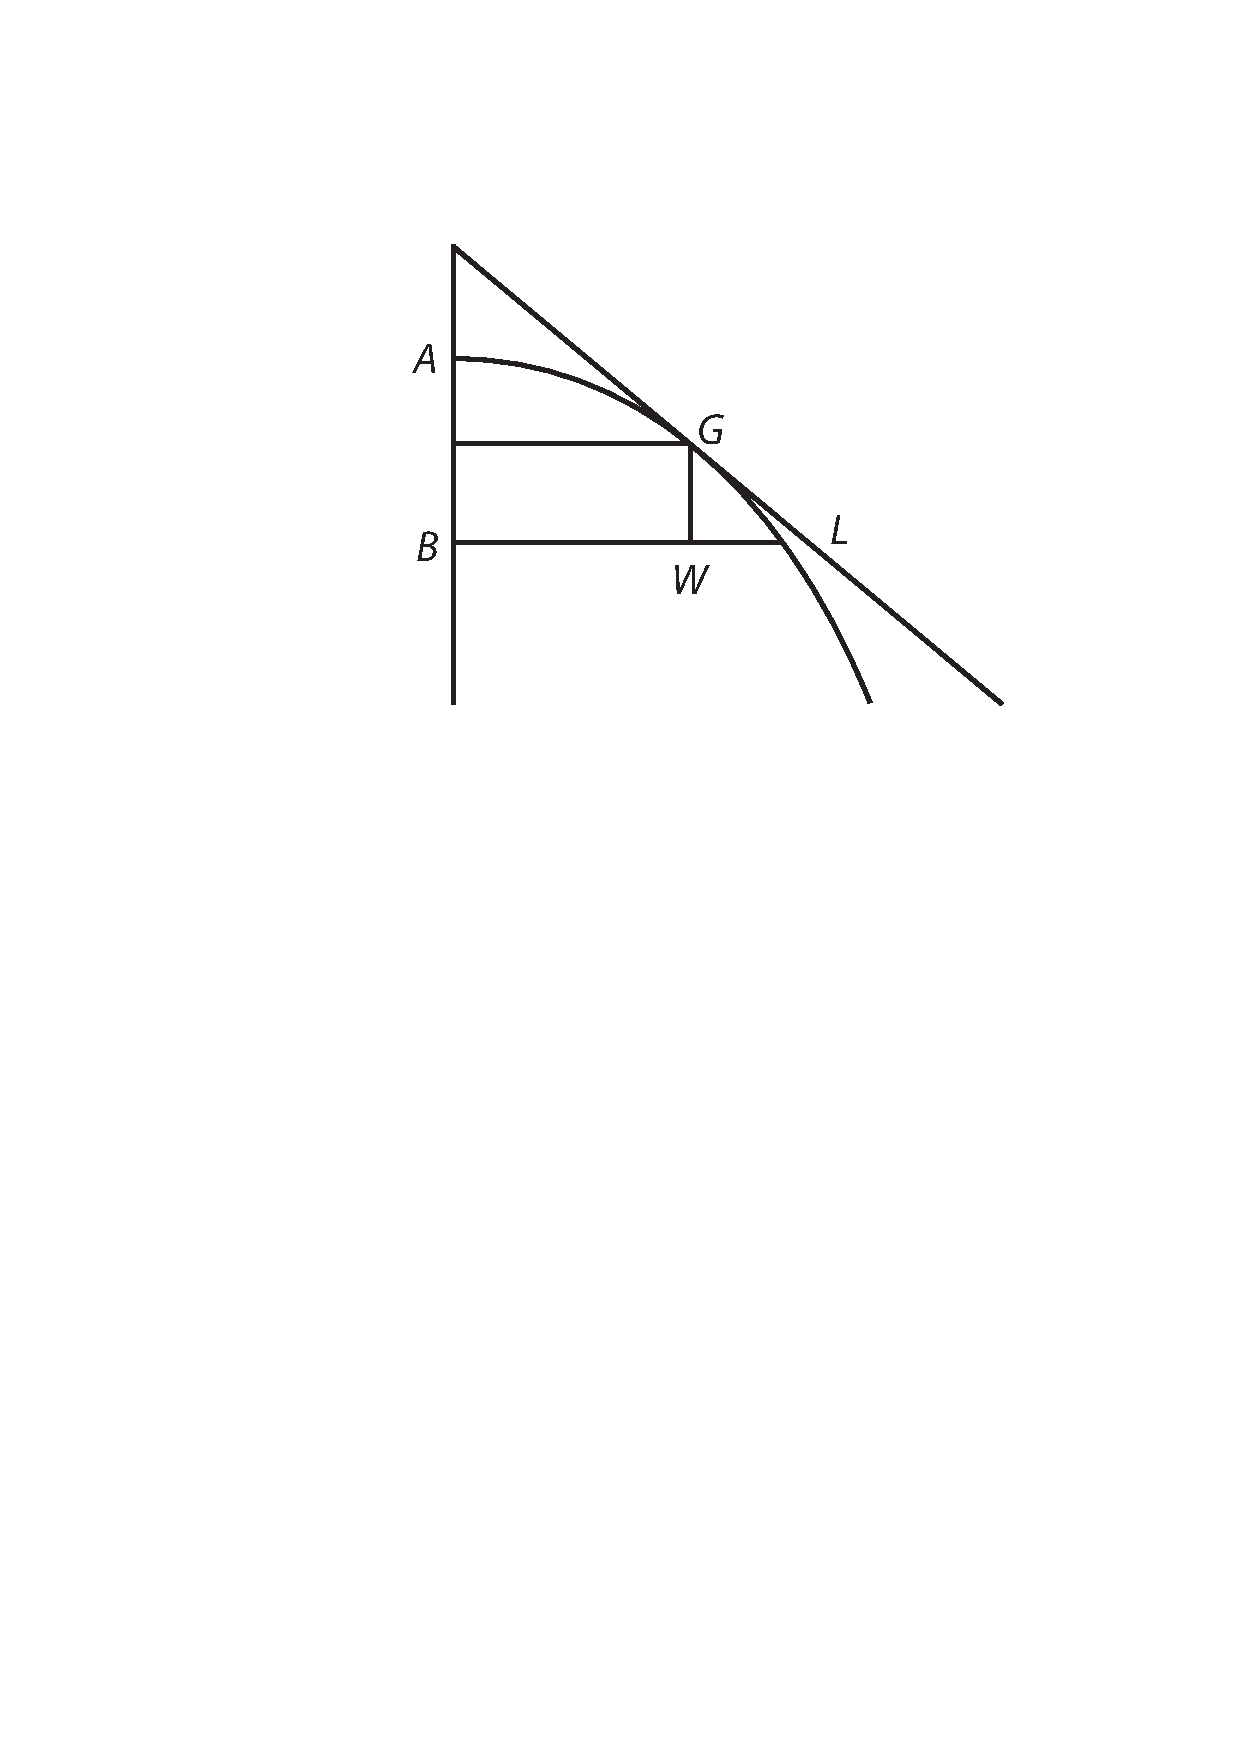
\includegraphics[width=0.28\textwidth]{images/lh0351303_035r-d3.pdf}\\
\rule[0cm]{13mm}{0cm}\textit{[Fig. 3]}
\end{wrapfigure}
\edtext{}{\Afootnote{\textit{Die Figur 3 einschlie{\ss}end und zwischen zwei Zeilen im Text, durch einen umlaufenden Strich vom Text abgetrennt}: $ \sqrt{1-y^{4}} $ Methodus generalis quadrandi figuram curvilineam quamlibet. Dato valore ipsius \textit{WL} per datam $ AB \, \sqcap \, x $ pro \textit{x}, substituatur alius valor; ut tunc \textit{WL} substituto eo valore fiat quadrabilis tunc compositione duorum motuum, uno in ipsius \textit{x} valore seu curvae ad quem est valor ille ordinatis, altero in ordinatas quadratricis ipsarum \textit{WL} \edtext{factitiarum}{\lemma{} \Bfootnote{ factitiarum \textit{erg.} \textit{ L}\ } uno transverso, altero recto habebitur descriptio quadratricis, valoris ipsarum \textit{WL} initio datarum unde facile est eligere constructiones simplicissimas, et infinitos eandem figuram describendi modos.}}} Sed si pro \textit{z} ponatur \( \displaystyle \dfrac{y^{2}\beta}{a^{2}}  \), fiet \( \displaystyle x \, \sqcap \, \dfrac{y^{3}}{3a^{2}}  \) et \( \displaystyle WL \, \sqcap \, \dfrac{3a^{3}\beta}{y\beta}  \).\\
Quanta sit vis percussionis a nemine satis explicatum arbitror. Pone grave\edtext{dati ponderis ex data altitudine super lancem}{\lemma{grave} \Bfootnote{ ex data altitudine \textit{ erg. } \textit{ L } \textit{ (1) }\ in \textit{ (a) }\ alteram \textit{ (b) }\ lanc \textit{ (c) }\ mo \textit{ (2) }\  dati ponderis  \textbar ex data altitudine \textit{erg.} \textbar super lancem \ \textit{ L } }} librae cadere, quaeritur, quoties suum pondus in altera librae lance elevare possit. Est haec quaestio inter mechanicarum maximas habenda. Hactenus enim vires mortuas, seu pondera, aut etiam vires vivas seu ictus inter se comparavere Geometrae, sed nunc primum vires mortuae vivis credo comparantur. \edtext{Vim autem}{\lemma{comparantur.} \Bfootnote{ \textit{ (1) }\ Sane \textit{ (2) }\ Vim autem \textit{ L }\ }} mortuam voco, ponderis quieti, qua elevationi suae aut loco motioni resistit; vivam vero, quam acceleratione successiva quaesivit. R. P. Kircherus\protect\index{Namensregister}{\textso  {Kircher}, Athanasius (1601-1680) SJ} alicubi \edtext{}{\lemma{alicubi: }\Cfootnote{Cf. A. Kircher SJ, Kurztitel und Jahr, S. xxx-xxx. ??}} meminit se expertum, 20 et ultra pilas, ab una ex mediocri distantia labente elevatas. Alii sibi persuasere inde duci posse perennem motum; \edtext{Galilaeus\protect\index{Namensregister}{\textso  {Galilei}, Galileo (1564-1642)}}{\lemma{motum;} \Bfootnote{ \textit{ (1) }\ vir quidam doctissimus conj \textit{ (2) }\ Galilaeus \textit{ L}\ }} et post eum Borellus\protect\index{Namensregister}{\textso  {Borelli}, Giovanni Alfonso (1608-1679)}, cum dixissent ictum esse infinitum,\edtext{}{\lemma{Galilaeus et post eum Borellus: }\Cfootnote{G. Galilei, Discorsi e dimostrazioni matematiche, Leiden 1638, S. 288 (GO VIII, S. 312f.); G. A. Borelli, De vi percussionis, Bologna 1667, proemium (nicht paginiert) und cap. 27-29 (S. 192-210).}} non ultra \edtext{}{\lemma{non ultra} \Bfootnote{ \textbar  tamen \textit{ gestr. }  \textbar  \textit{ L }\ }} explicuere, quasi proinde ulla inter vim mortuam et vivam comparatio cessaret, velut inter finitum et infinitum. Vir quidam nostris temporibus, in experimentis inveniendis et explicandis ingeniosissimus\protect\index{Namensregister}{\textso  {Mariotte}, Edme, Seigneur de Chazeuil (ca. 1620-1684)}, \edtext{sentit}{\lemma{ingeniosissimus} \Bfootnote{ \textit{ (1) }\ credit \textit{ (2) }\ sentit \textit{ L }\ }} guttam aquae lapsu suo praecise \edtext{cylindrum}{\lemma{praecise} \Bfootnote{ \textit{ (1) }\ guttam \textit{ (2) }\ cylindrum \textit{ L }\ }} aquae sustinere ejus altitudinis, unde lapsa est, et ejusdem cum gutta basis, unde negat vim ictus esse infinitam, aut certe tam magnam quam faciunt\edtext{}{\lemma{faciunt: }\Cfootnote{E. Mariotte, Trait\'{e} de la percussion ou choc des corps, Leiden 1717, S. 82.}}. Ego in hoc negotio investigando ita processi.\pend
\pstart  
\begin{wrapfigure}{l}{0.3\textwidth}
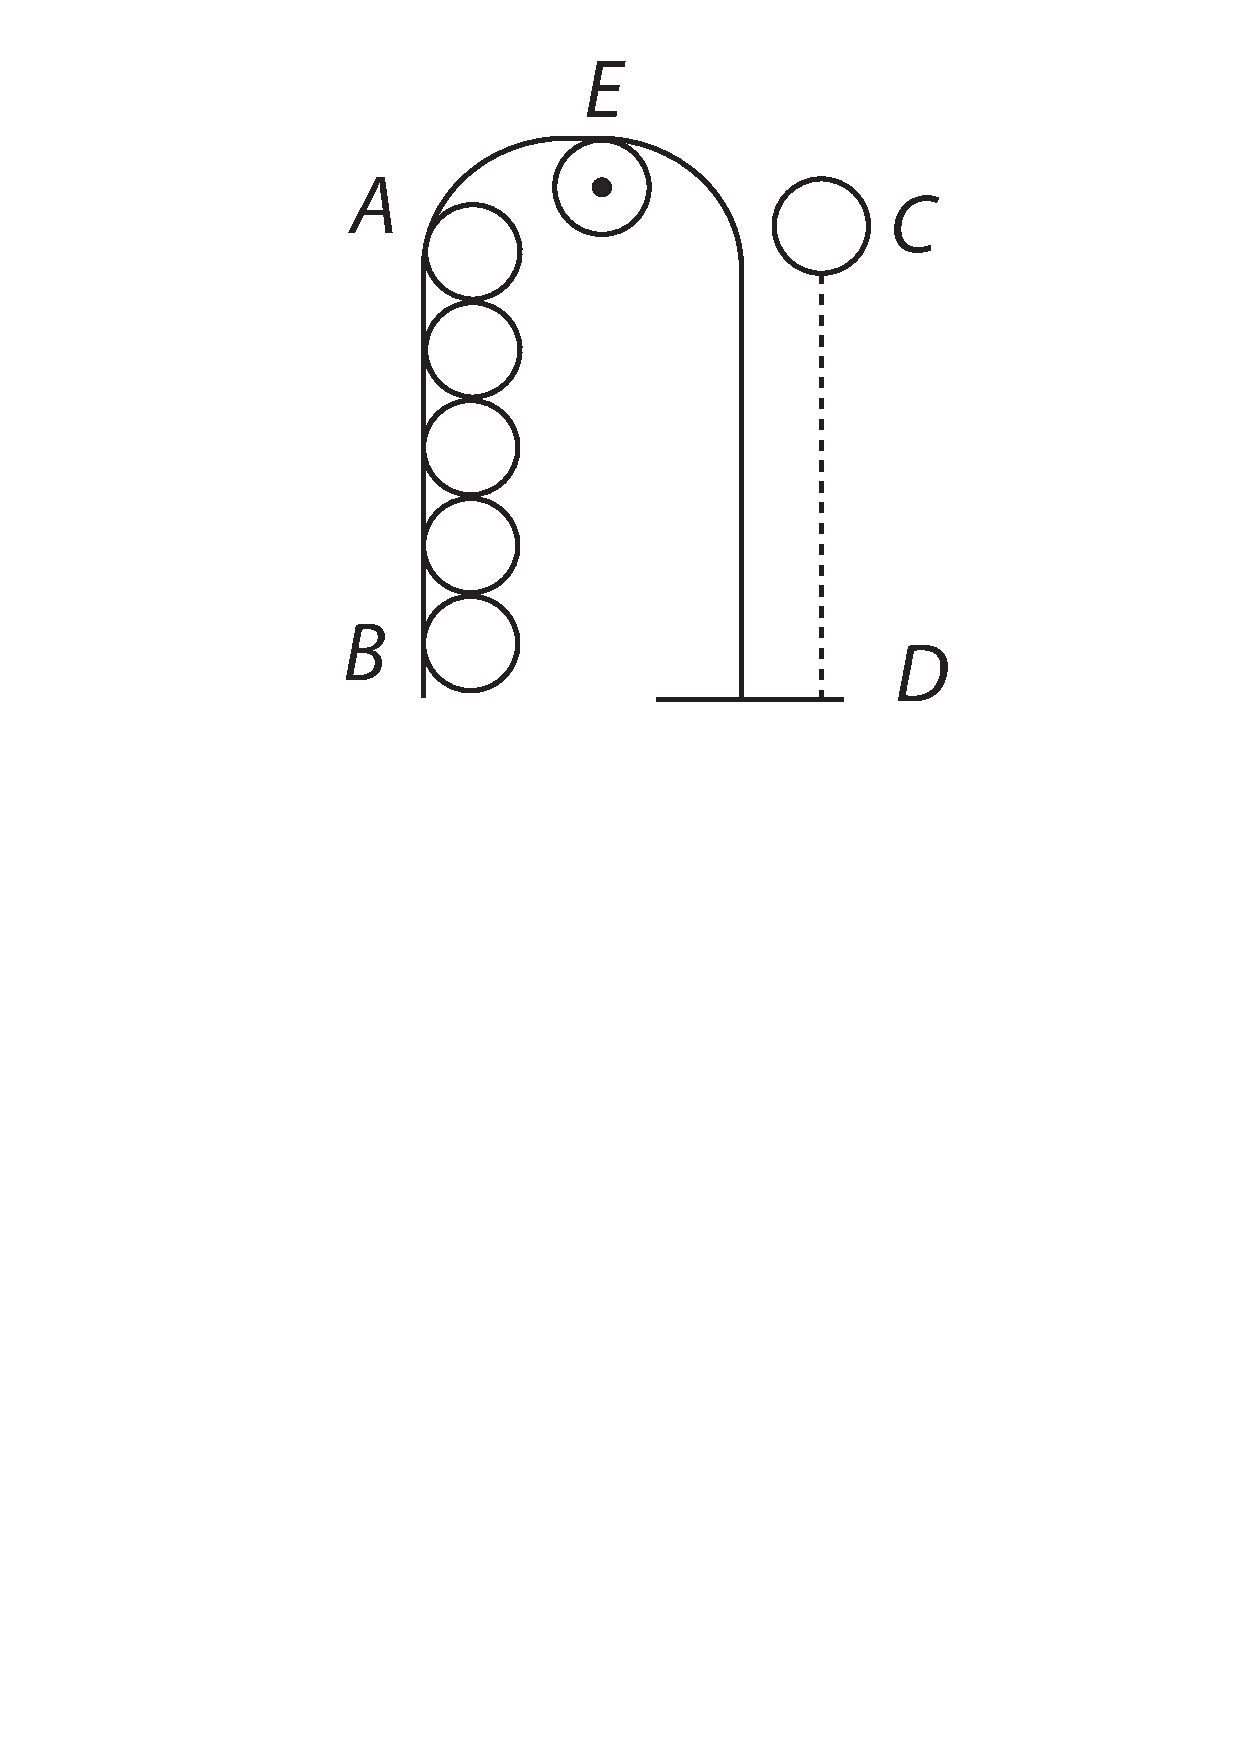
\includegraphics[width=0.27\textwidth]{images/lh0351303_035r-d4.pdf}\\
\rule[0cm]{12mm}{0cm}\textit{[Fig. 4]}
\end{wrapfigure}
Fingatur catena \edtext{globorum contiguorum}{\lemma{catena} \Bfootnote{ \textit{ (1) }\ corporum ita \textit{ (2) }\ globorum contiguorum \textit{ L }\ }} \textit{AB} unde summa \textit{C}, cadens in patinam \textit{D}, ope chordae \textit{DE} circa trochleam \textit{E}, faciat surgere catenam, et ipsa succedat in ultimae locum, summa autem rursus cadat succedatque in locum ipsius; patet inde sequi perennem motum. Quod est absurdum\edtext{;}{\lemma{absurdum}\Bfootnote{ \textbar ;  \textit{ erg. } \textbar patet  \ }} patet ergo non posse tantam esse vim ictus, quantam sufficit ad elevandam eousque catenam, ut \edtext{continuari possit}{\lemma{ut} \Bfootnote{ \textit{ (1) }\ attollere possit \textit{ (2) }\ continuari possit \textit{ L}\ }} ictus. Nimirum illud pro certo habendum est, solo lapsu fieri non posse, ut corpus labens, aut aliud ei aequipollens altius attollatur, quam unde lapsum est. Pone enim aequipollens altius attolli posse, sequitur ipsummet altius attolli posse; nam aequipollens altius sublatum cogatur in libram incidere, qua attollat datum; fiet, ut lapsus solus corporis dati, causa sit ascensus in locum ipso lapsu altiorem. Principium hoc tum rationibus tum experimentis confirmari potest; rationibus, quod natura non videatur agere contra se ipsam, experimento, quod pendulum sibi permissum numquam ad altitudinem priorem reascendit; cum tamen summa sit libertas ipsi; multo minus corpus ad altiorem sibi locum ascendet \edtext{per ipsam sui lapsus vim}{\lemma{ascendet} \Bfootnote{ \textit{ (1) }\ vi lap \textit{ (2) }\ per ipsam sui lapsus vim \textit{ L}\ }} in alia corpora transditam. Sed demonstratio hujus rei altior est, quod scilicet tam est facile attollere centum libras ad unam leucam, quam unam libram ad 100 leucas, tantundem enim effectus consecuta est rerum natura.\edtext{}{lemma{}\Afootnote{\textit{Zwischen den Zeilen, entgegen der Schreibrichtung und getilgt}: maxima pars hominum rudibus damnata tenebris.}}\pend
\pstart
Itaque in motibus illis universalibus infatigatis, ubi semper effectum suum quantum fieri potest, consequitur rerum natura.\hfill \\
\begin{wrapfigure}{l}{\textwidth}
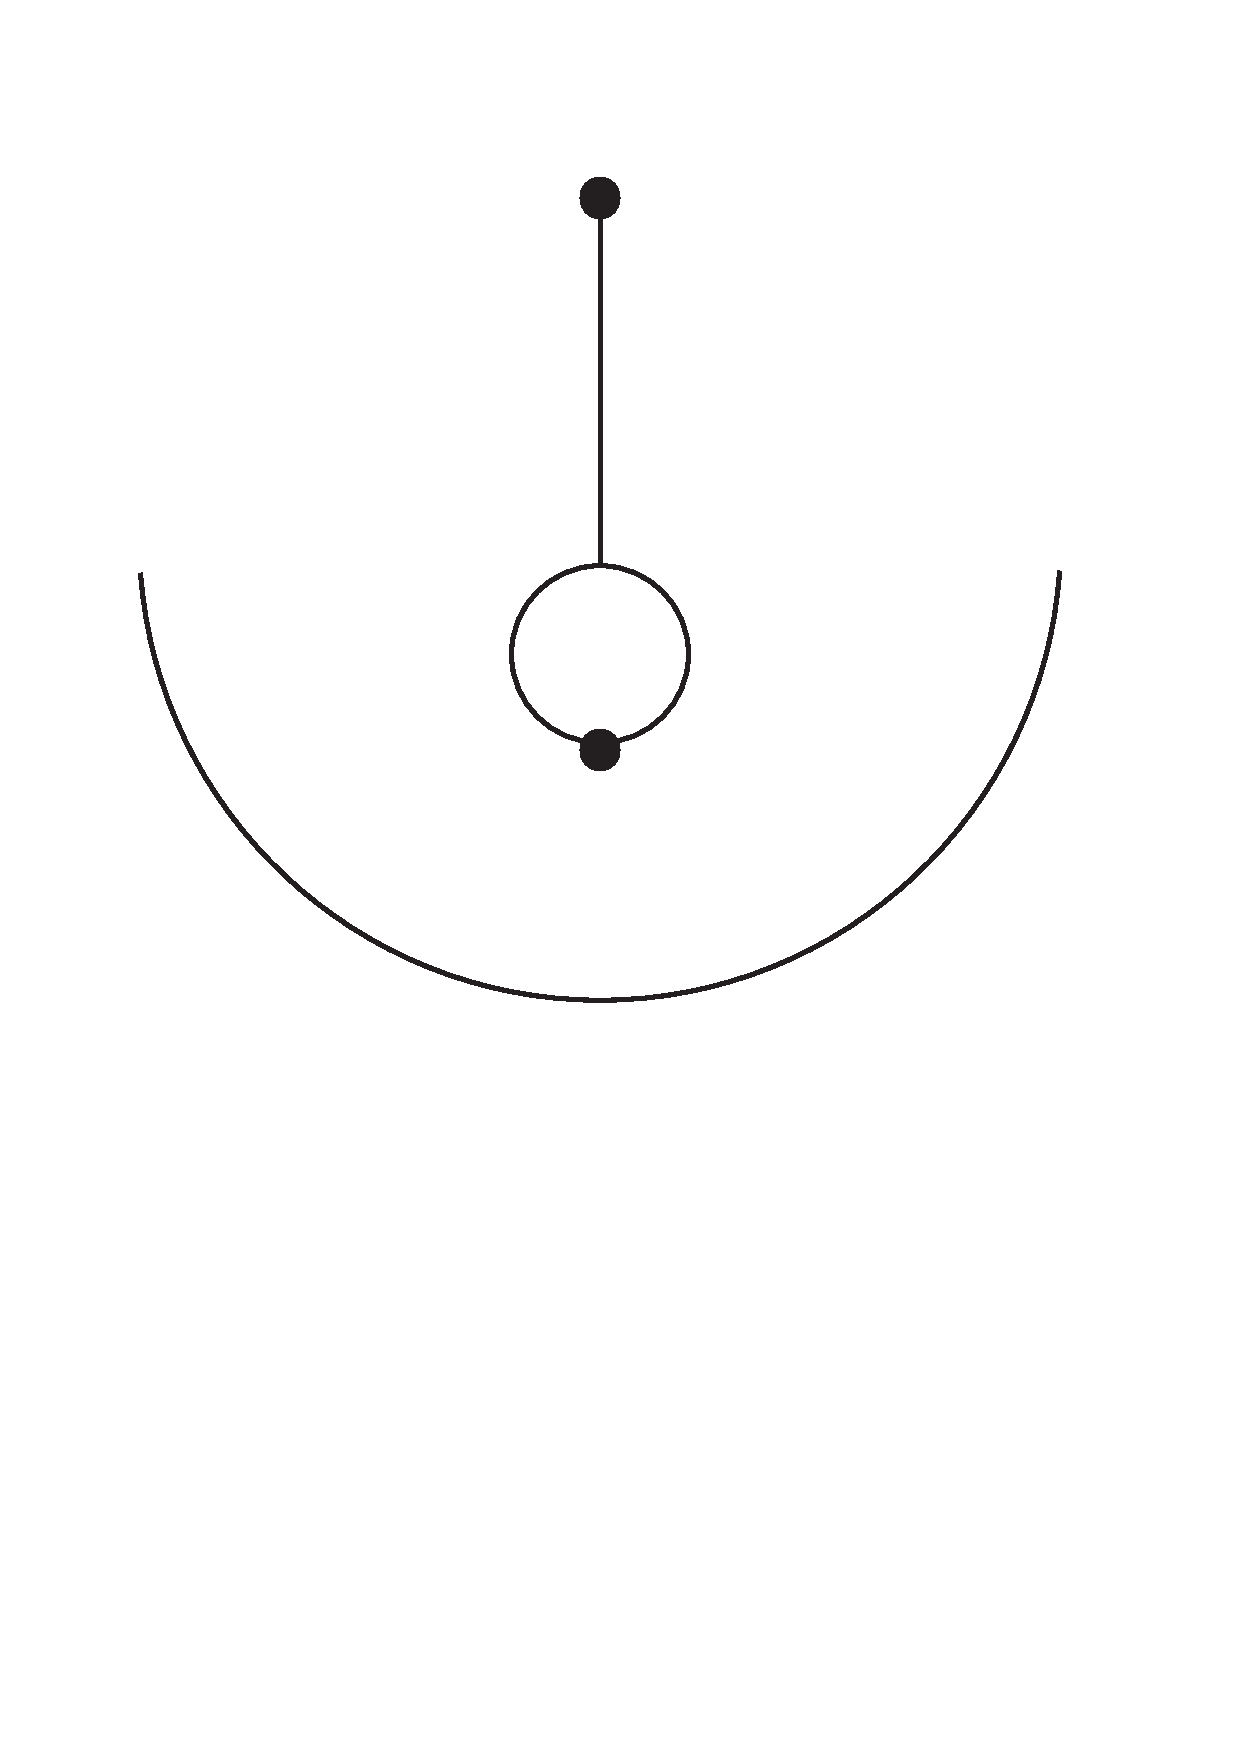
\includegraphics[width=0.2\textwidth]{images/lh0351303_035r-d5.pdf}\\
\rule[0cm]{5mm}{0cm}\textit{[Fig. 5]}
\end{wrapfigure}
\pend
 

